\chapter{Orçamento}

Para construir ou reformar é preciso conhecer as etapas de uma obra, desde a contratação dos projetos de arquitetura até a limpeza do local. O orçamento é uma das etapas de elaboração de um projeto de construção ou reforma.

O orçamento de obra é a etapa onde se estabelecem os custos envolvidos na execução da obra, especificando as atividades necessárias para a aplicação do projeto (comumente nomeadas de \emph{serviços}), se aprofundando nos custos envolvidos para a execução de cada atividade, desde mão-de-obra e custo de material básico como cimento e areia, da utilização de recursos externos tais como equipamentos alugados e até mesmo mão-de-obra especializada, impostos envolvidos nas atividades, entre outros.

Um projeto pode apresentar diversos orçamentos, comumente criados como estimativas e ajustados até que se chegue ao orçamento de venda. O orçamento de venda é o orçamento de custos reais (que irá ser aprovado em uma concorrência).
O responsável pela elaboração do projeto cria um orçamento que inicialmente é nomeado de orçamento de ``estimativa''. Um orçamento de estimativa serve como base para a criação do orçamento de ``venda'', e também para manutenção de histórico do projeto. Todos os orçamentos de estimativa criados para o projeto são mantidos. Após a aprovação de um orçamento e o início de execução do projeto é necessário realizar o acompanhamento do projeto, que é feito a partir do orçamento de ``execução''. O orçamento de execução é originado com base no orçamento de venda, podendo sofrer ajustes e aditivos \textbf{não} previstos no orçamento de ``venda''. Já ajustes realizados com base no desejo são realizados no orçamento de ``venda'' e refletidos automaticamente para o orçamento de ``execução''.

Portanto, existem 3 tipos diferentes de orçamento:

\begin{description}
	\item[Estimativa] \hfill \\
	Esboços de orçamentos para o projeto (histórico do projeto);
	\item[Venda] \hfill \\
	Orçamento inicial com base no histórico; e
	\item[Execução] \hfill \\
	Orçamento guia de execução do projeto.
\end{description}

\section{Orçamento de Estimativa}

Este é o orçamento impreciso, estimado, quando um cliente solicita um orçamento prévio para realização de um determinado serviço, sendo esse somente uma estimativa pois, neste momento, não há um projeto definido, não se conhecem todas as atividades necessárias para sua execução - somente atividades básicas e não complexas.

Normalmente na fase de estimativa levam-se em conta projetos base \footnote{projetos criados para servir de base para outros, tendo pequenas diferenças em suas atividades} para facilitar a recuperação de atividades padronizadas, sendo modificadas somente algumas atividades em particular ao projeto que se estima ou a quantidade do serviço para o projeto em questão. Além de utilizar projetos base, mais comumente são utilizados padrões de projetos (apostilas que determinam os elementos base de um determinado projeto). Nesses casos, o usuário que define o projeto deverá seguir os padrões pré-estabelecidos para manter a conformidade de suas atividades.

\section{Orçamento de Venda}

Nesta fase, o orçamento é baseado em projeto bem definido pelo engenheiro, tendo suas atividades bem definidas, todos os custos diretos e indiretos de execução do projeto definidos.
A obtenção do custo real é baseada na estruturação dos serviços e suas composições (veremos o que são composições mais adiante), determinadas pela quantidade de cada item para a execução do serviço, como mostra a figura \ref{fig:composicao}.

\begin{figure}[htb]
	\centering
	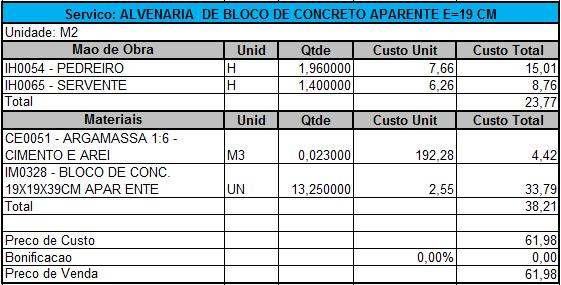
\includegraphics[width=0.9\textwidth]{figuras/composicao.jpg}
	\caption{Composição de um serviço}
	\label{fig:composicao}
\end{figure}

A definição do custo é a somatória de todos os recursos desprendidos na execução do projeto (custos diretos) e de todos os custos indiretos envolvidos.

Para o orçamento de venda, ainda constam os impostos e encargos sociais envolvidos e o lucro desejado com a execução do projeto (BDI).

Esse é o orçamento que é utilizado para \emph{vender o projeto} ao cliente. Após aprovado, o passo seguinte é acompanhar a execução do projeto com o orçamento de ``execução''.

\section{Orçamento de Execução}

Este orçamento, originado de um orçamento prévio de venda, recebe o realizado durante o projeto, provendo um comparativo futuro entre o que foi orçado e o que realmente foi executado. 

No orçamento de execução comumente surgem imprevistos que são registrados para reportar os custos reais do realizado e que não fora previsto pelo orçamento de venda. A figura \ref{fig:curva_abc} demonstra uma forma de comparativo entre ``previsto x realizado''.


\begin{figure}[htb]
	\centering
	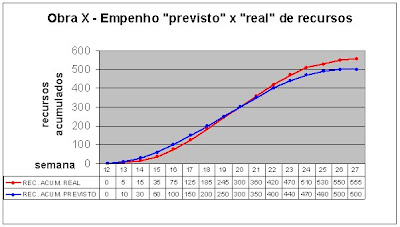
\includegraphics[width=0.9\textwidth]{figuras/curva_abc.jpg}
	\caption[Curva ABC]{Previsto x Realizado}
	\label{fig:curva_abc}
\end{figure}